\documentclass[]{beamer}
\usepackage{color}
\usepackage{listings}
\usepackage{verbatim}
\usepackage{graphicx}
\usepackage{multicol}
\usepackage[utf8]{inputenc}
\usepackage{amsmath}
\usepackage{graphicx}
\usetheme{Madrid}
\title{Bachelor-Thesis}
\subtitle{Simulation of the RoboCup Logistic League with Fawkes and Gazebo for Multi-Robot Coordination Evaluation}
\author {Frederik Zwilling}
\institute{RWTH Aachen}
\date{19.12.2013}
\subject{Multi-Robot Simulation}

%hide nav bar
\setbeamertemplate{navigation symbols}{}

\begin{document}
\frame{\titlepage}

%Beans
\begin{frame}
  \frametitle{The thesis at a glance}
  \begin{columns}
  \column[]{0.45\textwidth}
  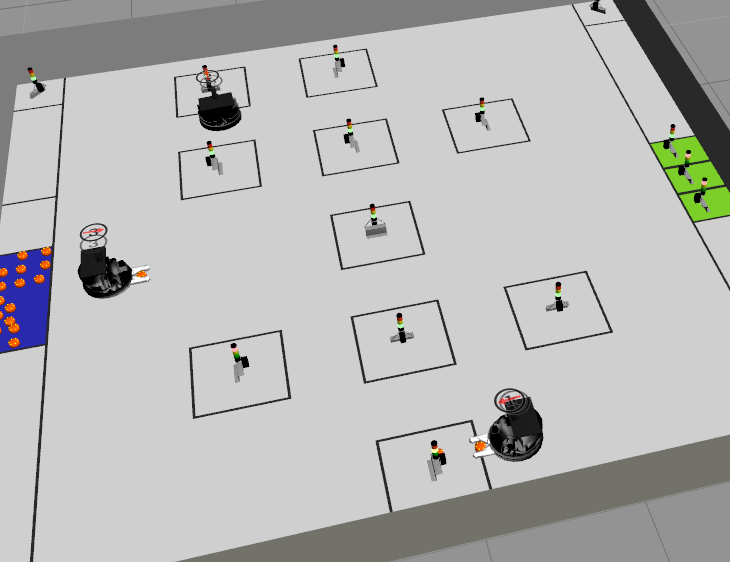
\includegraphics[width=\textwidth]{../pics/sim_working_small.png}
  \column[]{0.55\textwidth}
  \textbf{\large Multi-robot simulation}
    \begin{itemize}
    \item \textbf{Environment:} Physically and visually realistic
    \item \textbf{Domain:} RoboCup Logistic League
    \item \textbf{Purpose:} Testing and evaluating to improve our real system
    \item \textbf{Focus:} Agent coordination and high level control
    \end{itemize}
  \end{columns}
\end{frame}

%% %Schedule
%% \begin{frame}
%%   \frametitle{Schedule}
%%   \begin{enumerate}
%%   \item Motivation
%%   \item Background
%%   \item Related Work
%%   \item Approach
%%   \item Implementation
%%   \item Evaluation
%%   \item Summary
%%   \end{enumerate}
%%   \textcolor{red}{leave off slide?}
%% \end{frame}

%Motivation
\begin{frame}
  \frametitle{Motivation: Multi-Robot Systems and Logistics}
  \begin{columns}
    \column[]{0.45\textwidth}
    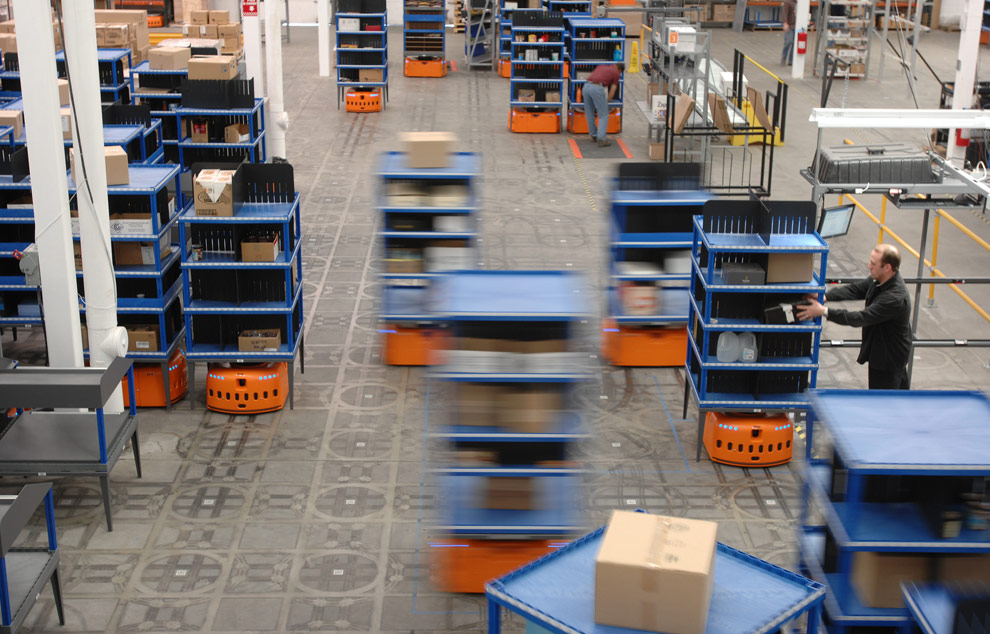
\includegraphics[width=\textwidth]{../pics/kiva.jpg}
    \column[]{0.55\textwidth}
    \textbf{\large Advantages of multi-robot systems:}
    \begin{itemize}
    \item Flexibility, parallelism
    \item Heterogeneous groups %Division of labour, specializing
    \item Many possible applications %Warehousing, Logistics
    \end{itemize}
    \textbf{\large Challenges:}
    \begin{itemize}
    \item Complexity
    \item High effort of testing and evaluating
    \end{itemize}
  \end{columns}
\end{frame}

\begin{frame}
  \frametitle{Motivation: Simulation}
  \textbf{\large Advantages of a simulation:}
  \hspace{2cm}\\
  \begin{itemize}
  \item Possibility to test without real environment and robots
  \item Fast execution of test, automated test runs
  \item Testing on different abstraction levels
  \item Easy comparison of performance with different configurations 
  \item Especially large advantage for multi-robot systems
  \end{itemize}
\end{frame}

%%%% Background %%%%
\begin{frame}
  \frametitle{Logistic League sponsored by Festo (LLSF)}
  \fboxsep=0pt
  \noindent
  \begin{minipage}[]{0.48\linewidth}
    \begin{figure}
      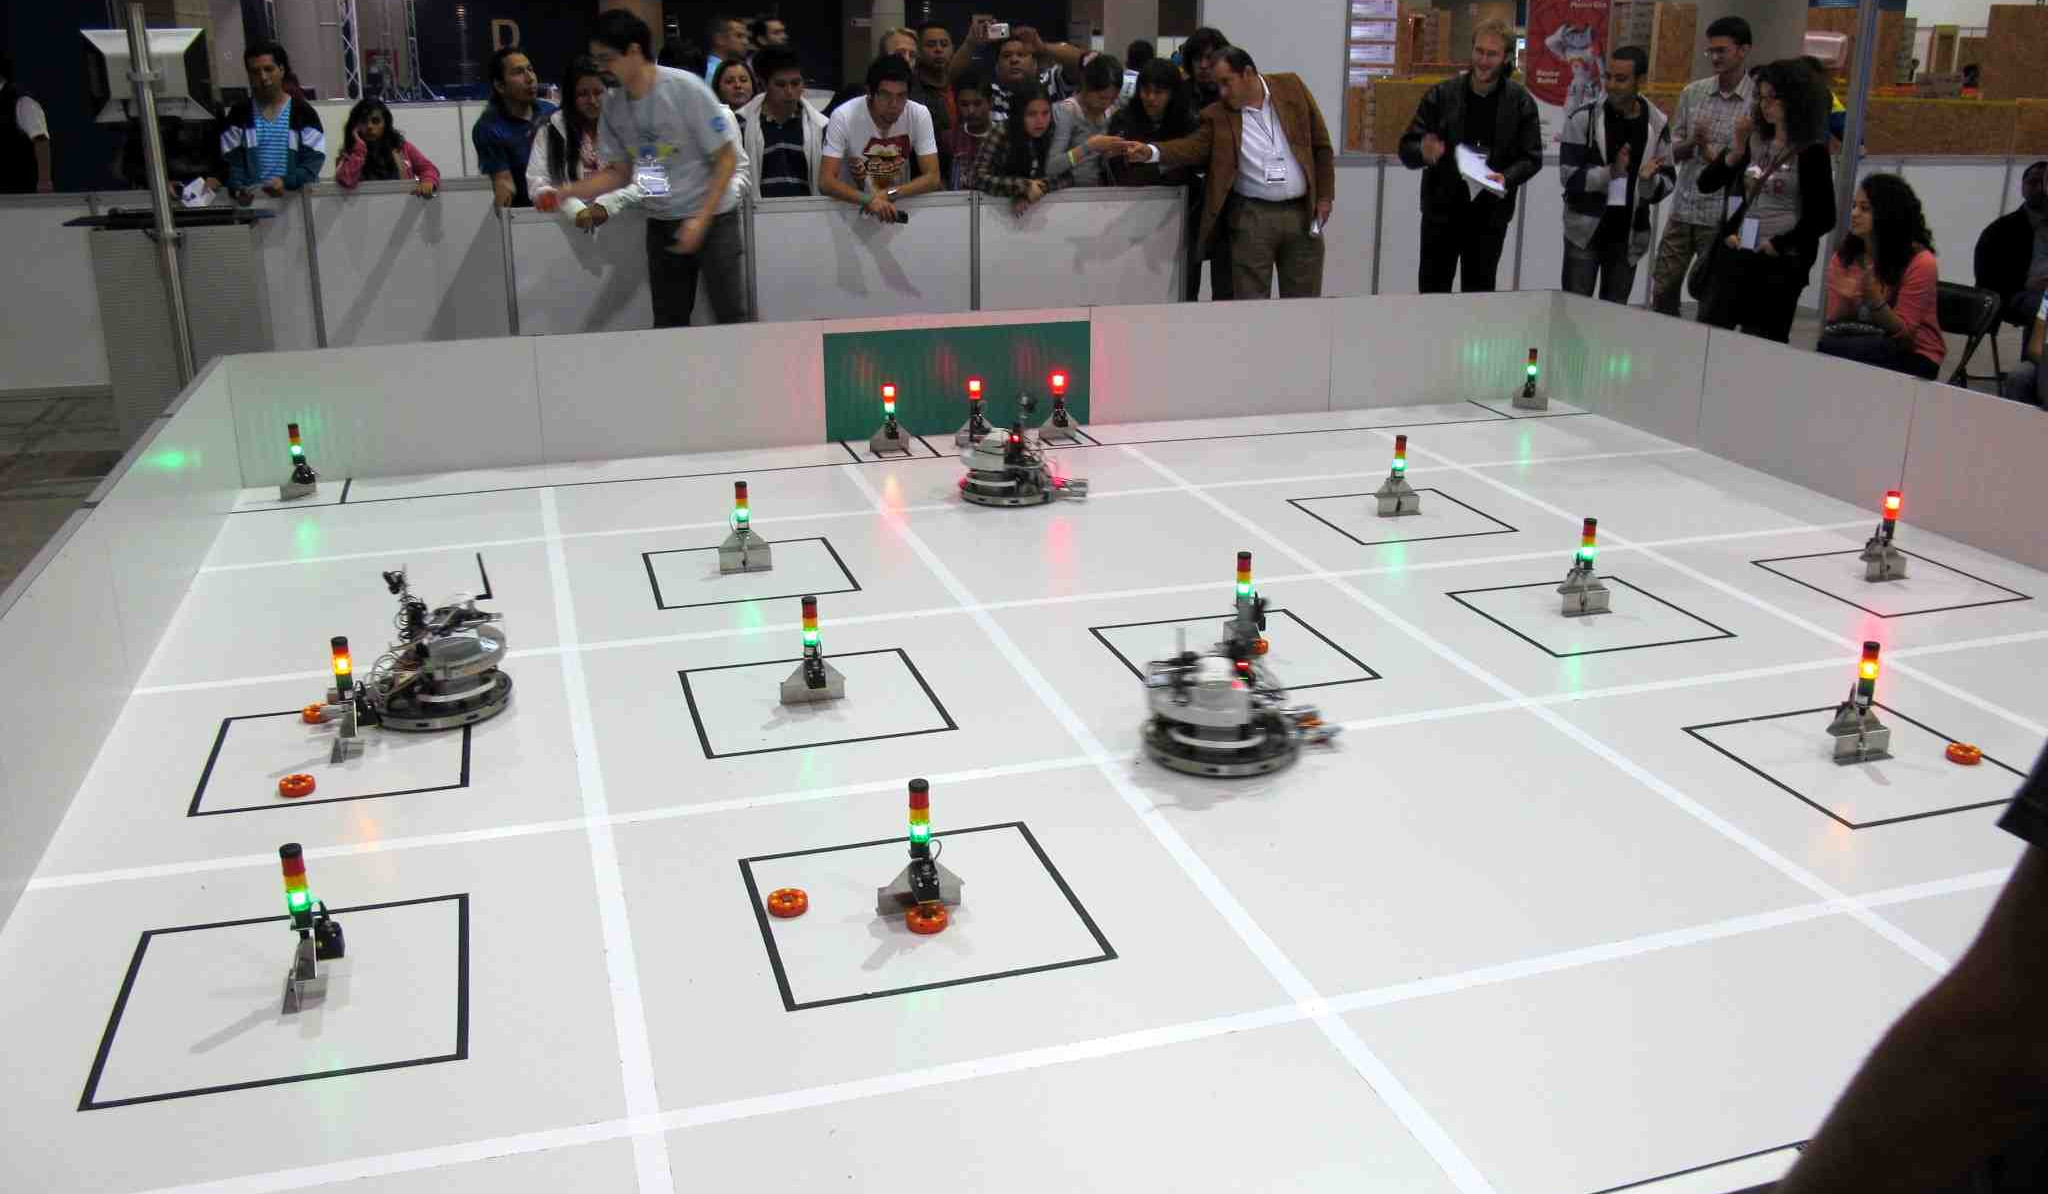
\includegraphics[width=\textwidth]{../pics/llsfLeague.png}\\
    \end{figure}
  \end{minipage}
  \hfill
  \begin{minipage}[]{0.48\linewidth}
    \textbf{\large League:}
    \begin{itemize}
    \item Part of RoboCup competition
    \item Testbed for logistic robots in a competitive factory automation scenario
    \end{itemize}
    \pause
    \textbf{\large Task:}
    \begin{itemize}
    \item Produce and deliver products by feeding machines% with resources and semi-finished products
    \item Optimize work-flow and performance of the system
    \item Being robust against failure
    \end{itemize}
  \end{minipage}
\end{frame}

\begin{frame}
  \frametitle{Fawkes}
  \begin{multicols}{2}
    \begin{figure}
      \only<1>{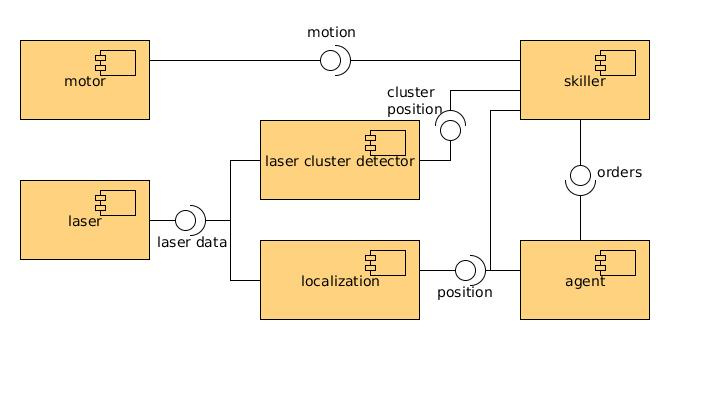
\includegraphics[scale=0.25]{../pics/simplefawkes.jpg}}
      \only<2>{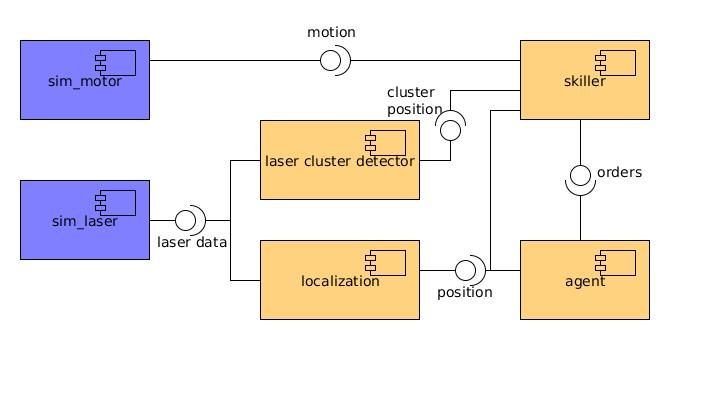
\includegraphics[scale=0.25]{../pics/lowsim.jpg}}
    \end{figure}
    \textbf{\large An Open Source robot software framework}
    \begin{itemize}
    \item Component-based software design
    \item Components are realized as plugins with multiple threads
    \item Blackboard communication infrastructure
      \pause
    \end{itemize}
  \end{multicols}
  \begin{itemize}
  \item[$\Rightarrow$] Easy exchange of sensor/actuator plugins by simulation plugins
  \end{itemize}
\end{frame}

\begin{frame}
  \frametitle{Gazebo}
  \begin{multicols}{2}
    \begin{figure}
      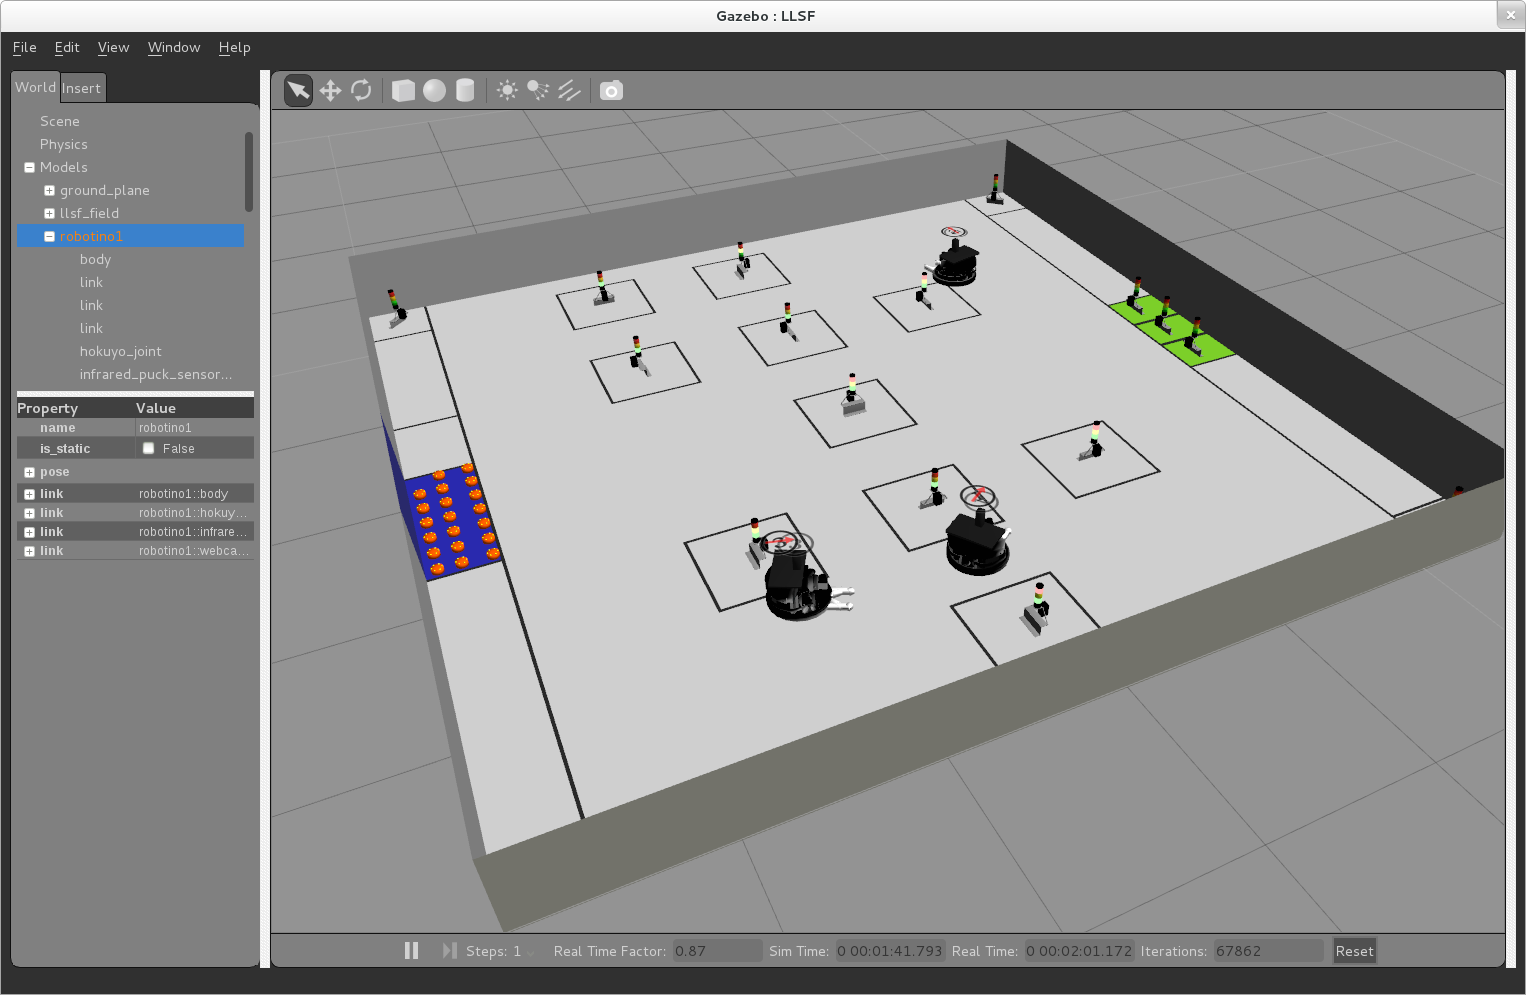
\includegraphics[scale=0.11]{../pics/gazebo_window.png}
    \end{figure}
    \textbf{\large An Open Source robot simulator}
    \begin{itemize}
    \item Powerful graphics and physics engines %Reflections, Slippery (Odom)
    \item Already supports some robots and sensors (e.g. Hokuyo laser sensor)
    \item Extensive support
    \end{itemize}
  \end{multicols}
\end{frame}

%%%% Related Work %%%%
\begin{frame}
  \frametitle{Related Work}
  \begin{multicols}{2}
    \only<1>{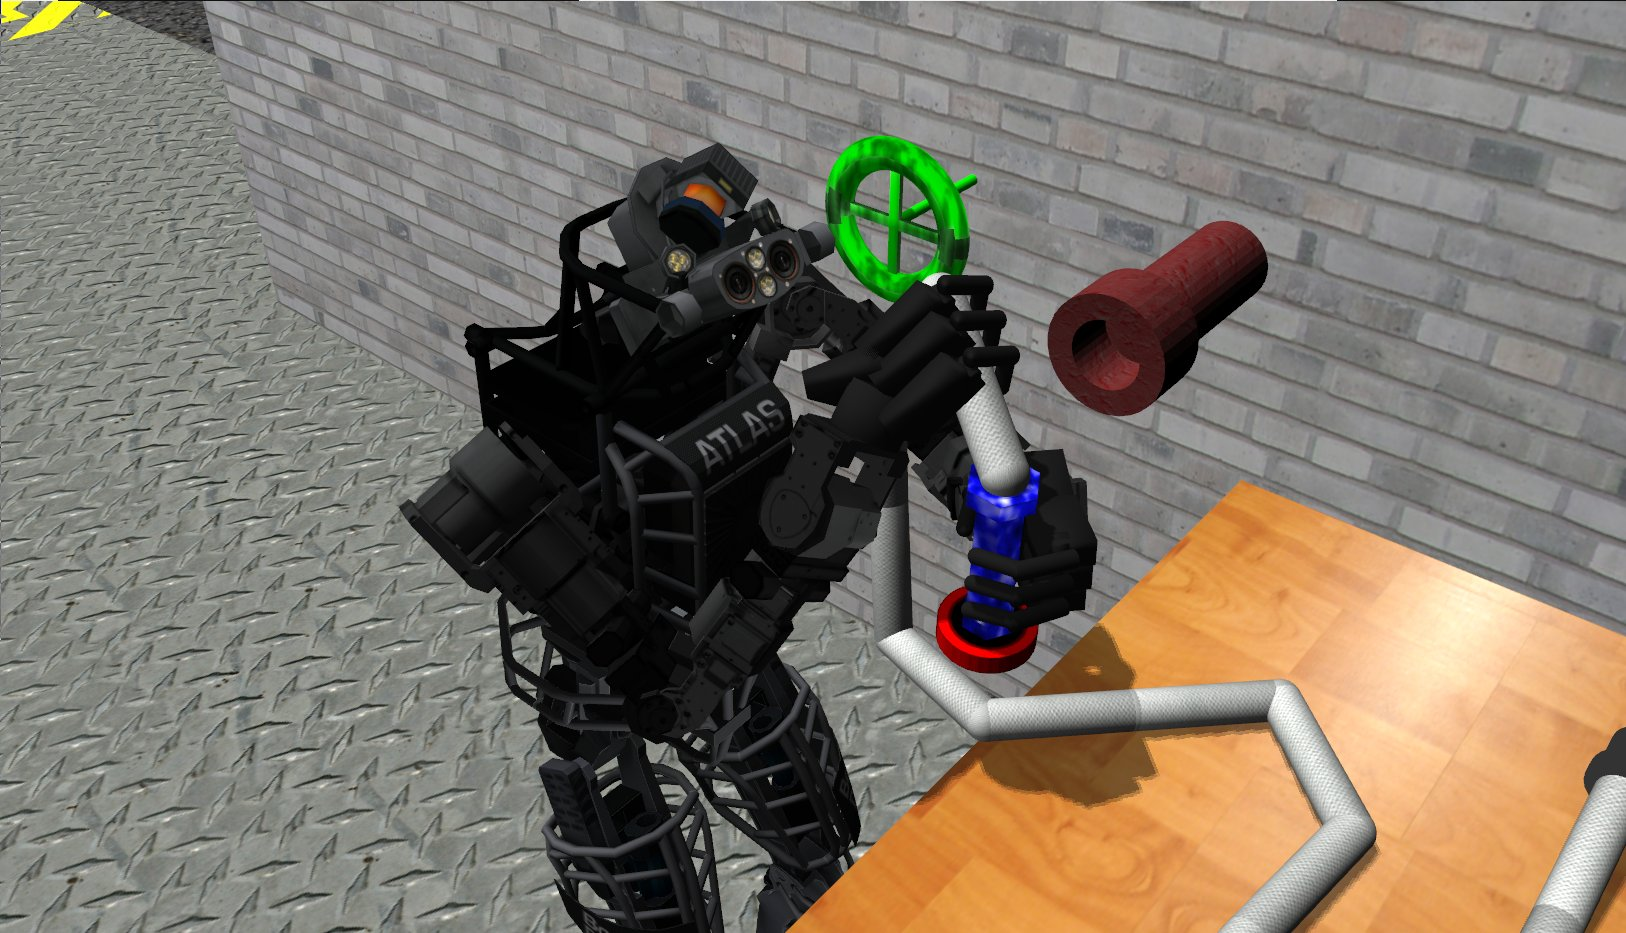
\includegraphics[width=0.52\textwidth,height=0.3\textwidth]{../pics/gazebo.jpg}}
    \only<2>{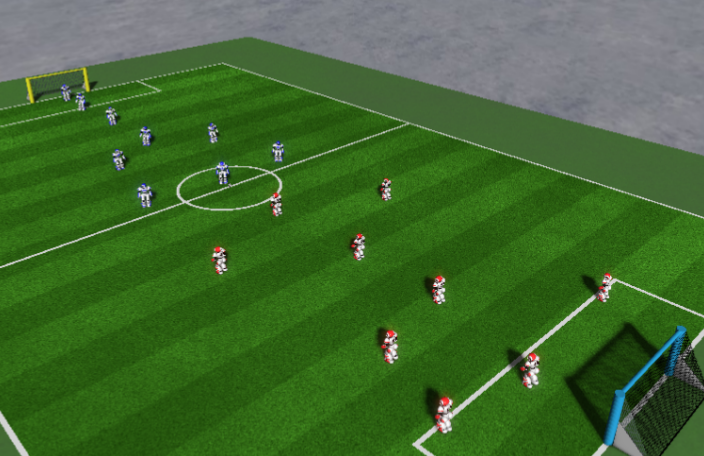
\includegraphics[width=0.52\textwidth,height=0.3\textwidth]{../pics/soccer_simulation_3d.png}}
    \only<3>{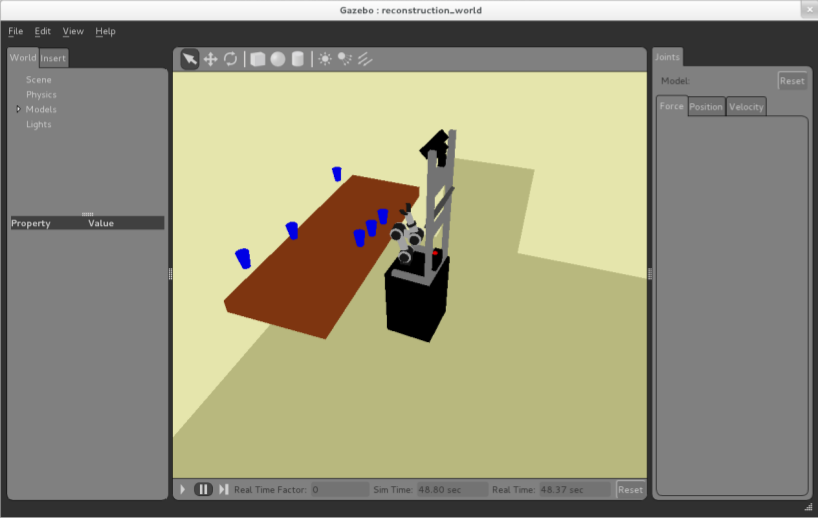
\includegraphics[width=0.52\textwidth,height=0.3\textwidth]{../pics/klingen_sim.png}}
    \only<4>{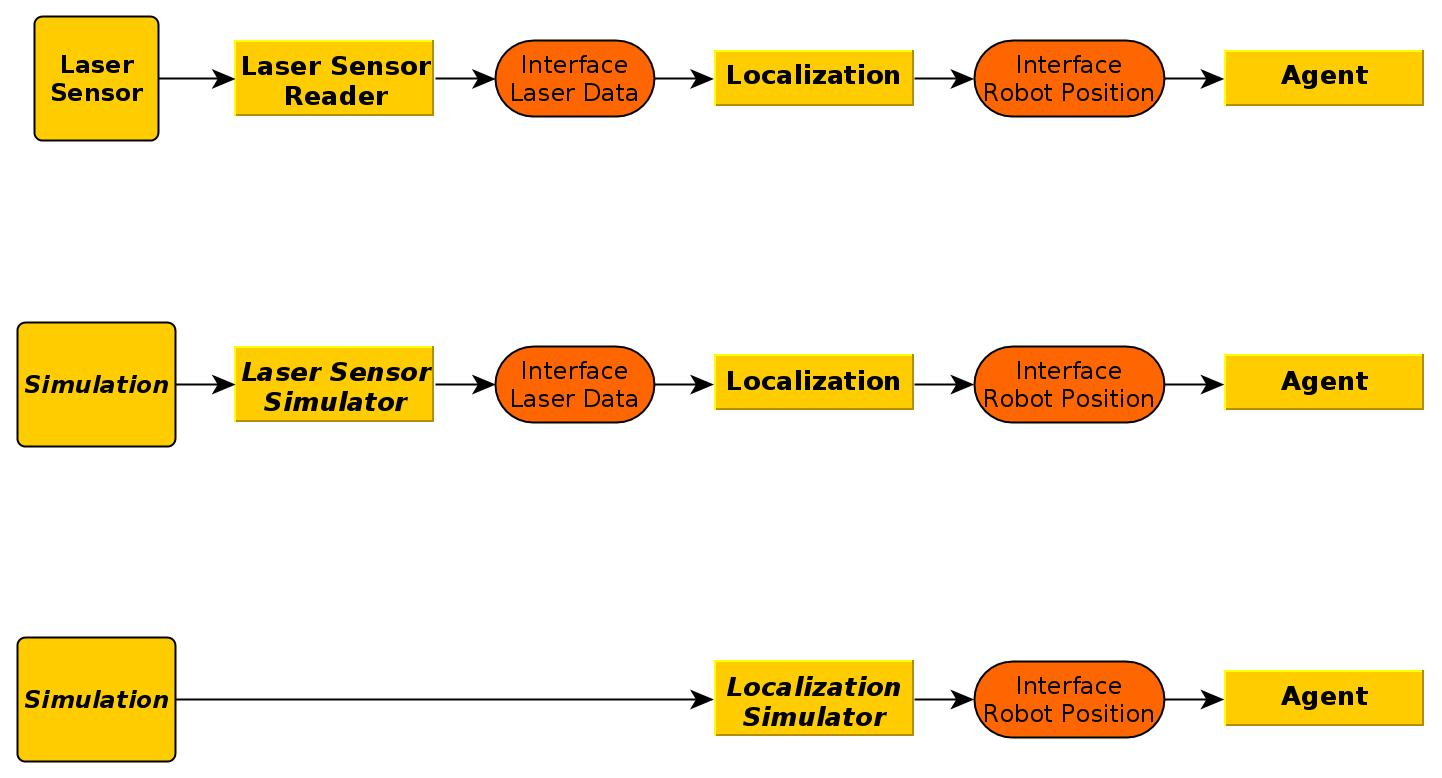
\includegraphics[width=0.52\textwidth,height=0.3\textwidth]{../tabs/mla_complete.jpg}}
    
    \begin{overlayarea}{0.52\textwidth}{.5\textheight}
      \begin{itemize}
      \item Virtual Robotics Challenge
        \pause
      \item RoboCup Simulation Leagues
        \pause
      \item Scene Reconstruction for Fault Analysis
        \pause
      \item Multi-Level Abstraction
      \end{itemize}
    \end{overlayarea}
  \end{multicols}
\end{frame}

%%%% Approach %%%%
\begin{frame}
  \frametitle{Approach}
  \begin{tabular}{p{3.7cm}|p{7.5cm}}
    \hline
    \large{\textbf{Goal}} & \large{\textbf{Approach}}\\
    \hline
    Realistic simulation & \begin{itemize} \item Using Gazebo \item Sensors with noise \end{itemize} \pause \\ %Using Gazebo, \newline Sensors with noise \pause \\ 
    \hline
    Individual testing of high-level components & \begin{itemize} \item Multi-Level Abstraction \end{itemize} \pause \\ %Multi-Level Abstraction \pause \\
    \hline
    Efficient testing & \begin{itemize} \item Start-up scripts \item Loading different configurations \item Visualizing robot belief \end{itemize} \pause \\ %Start-up scripts, \newline Loading different configurations, \newline Visualizing robot belief \pause\\ 
    \hline
    Multi-robot system evaluation & \begin{itemize} \item Scheduling simulation runs \item Performance statistics and recording \end{itemize} \pause \\ % Scheduling simulation runs, \newline Performance statistics and recording \pause\\    
    \hline
    Expandability & \begin{itemize} \item Small and reusable modules \end{itemize} \pause \\ %Small and reusable modules \pause\\
    \hline
    Agent improvements & \begin{itemize} \item Using three robots \item Recycling \item Dynamic role change \end{itemize} \pause \\ %Using three agents, \newline Recycling, \newline Dynamic role change\\
    \hline    
  \end{tabular}
\end{frame}


\begin{frame}
  \frametitle{Architecture: Simulation}
  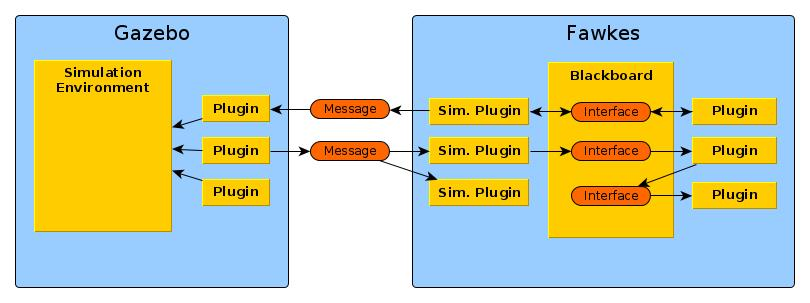
\includegraphics[width=\textwidth]{../tabs/fawkes_gazebo.jpg}
\end{frame}

\begin{frame}
  \frametitle{Architecture: Communication}
  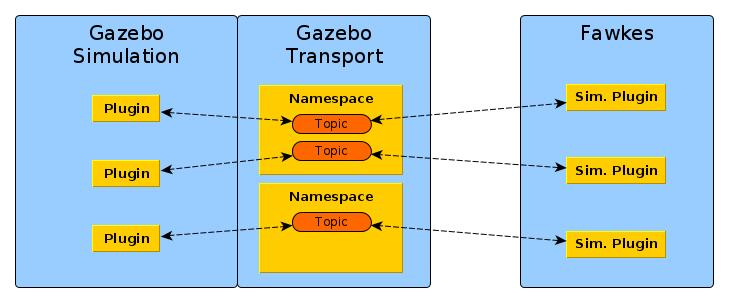
\includegraphics[width=\textwidth]{../tabs/communication.jpg}
\end{frame}

%%%% Implementation %%%%
\begin{frame}
  \frametitle{Implementation}
    \begin{itemize}
    \item Simulation models
      \begin{itemize}
      \item Field, Machines, Pucks
      \item Robotino
      \end{itemize}
    \item Gazebo Plugins
      \begin{itemize}
      \item World (LLSF game logic)
      \item Robotino (sensors, motor)
      \end{itemize}
    \item Fawkes Plugins
      \begin{itemize}
      \item Access to Gazebo
      \item Robotino (e.g. motor, gyro) 
      \item Sensors (high/low level)
      \item Organizational plugins (e.g. time-sync, inter-robot communication) %Time sync, Communication between robots, Visualizations, Statistics
      \end{itemize}
    \item Agent improvements
    \item Automation scripts
    \end{itemize}
\end{frame}

%%%% Evaluation %%%%
\begin{frame}
  \frametitle{Evaluation: Simulation}
  \textbf{\large Realism:}\\
  %no common measurement => evaluation of components
  \begin{itemize}
  \item LLSF can be simulated realistically
  \item Visualization sufficient for vision tasks %show vision
  \item Reflections and lightening conditions difficult to simulate %shows limitations
  \item Difficult to find good friction parameters
  \item[$\Rightarrow$] Many real problems can be simulated
  \end{itemize}
\end{frame}

\begin{frame}
  \frametitle{Evaluation: Hackathon}
  \begin{multicols}{2}
    \center
    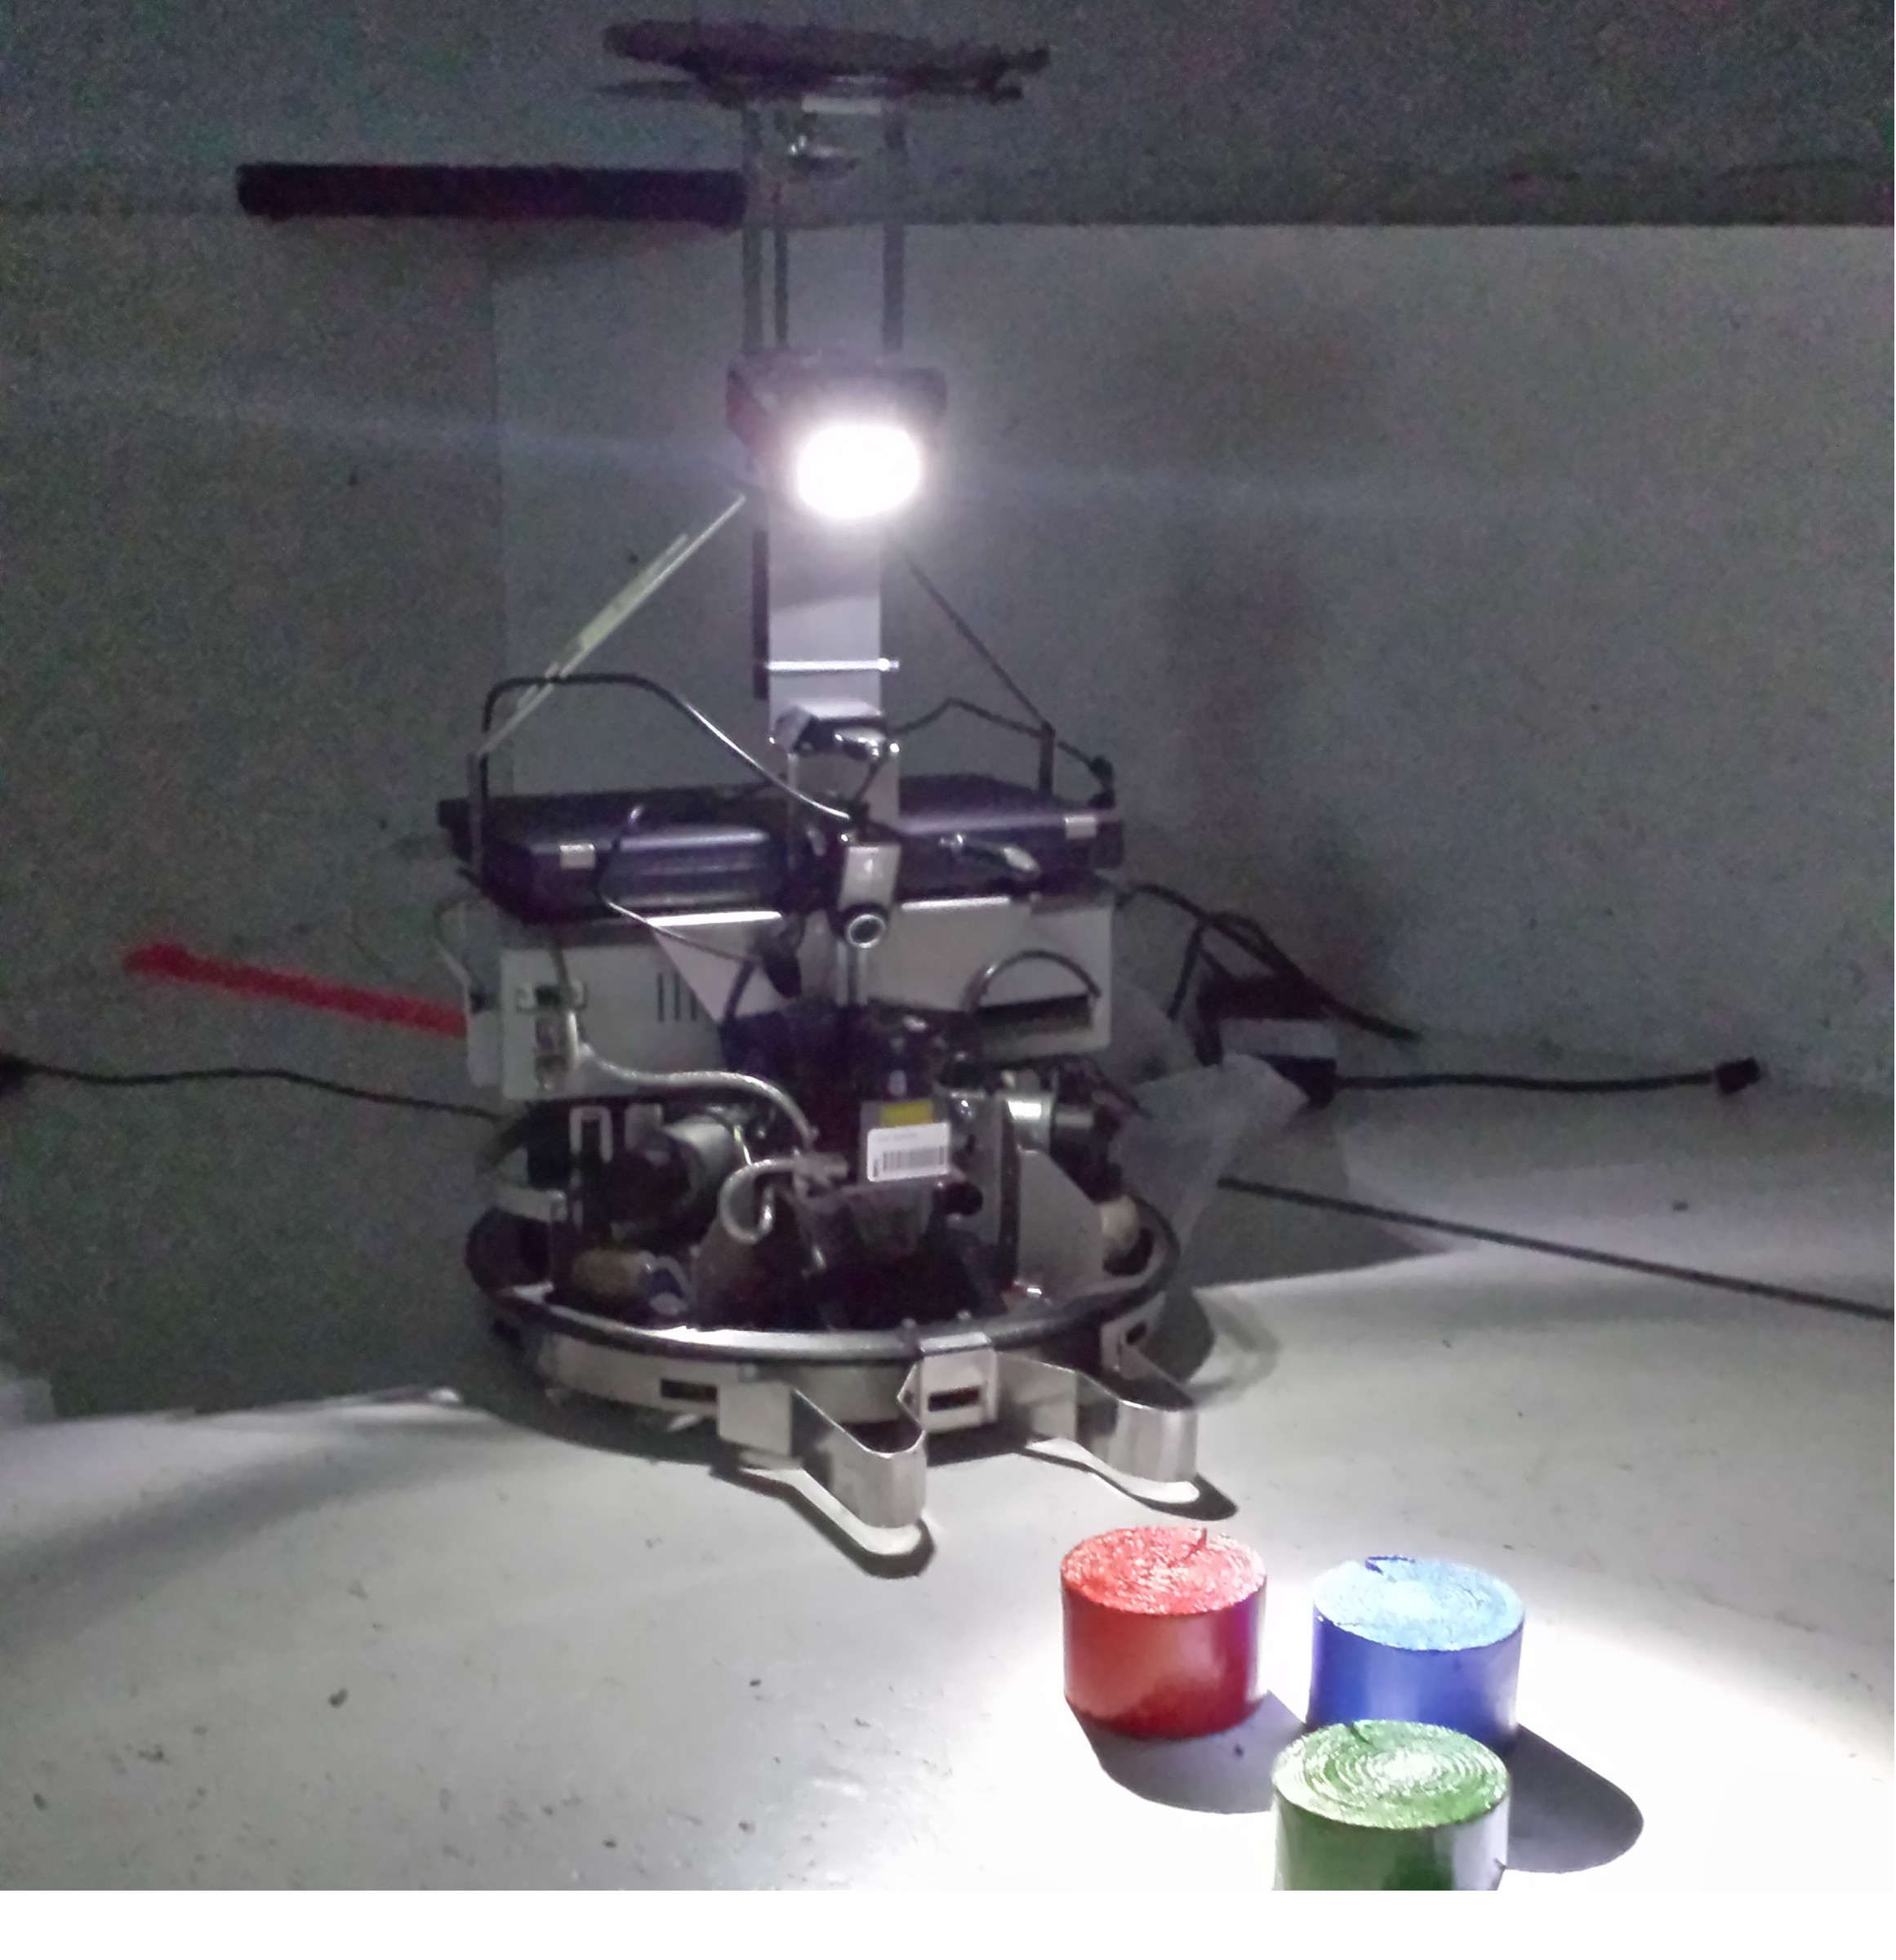
\includegraphics[width=0.3\textwidth]{../pics/hackathon_real_de}\\
    \hspace{0.5cm}\\
    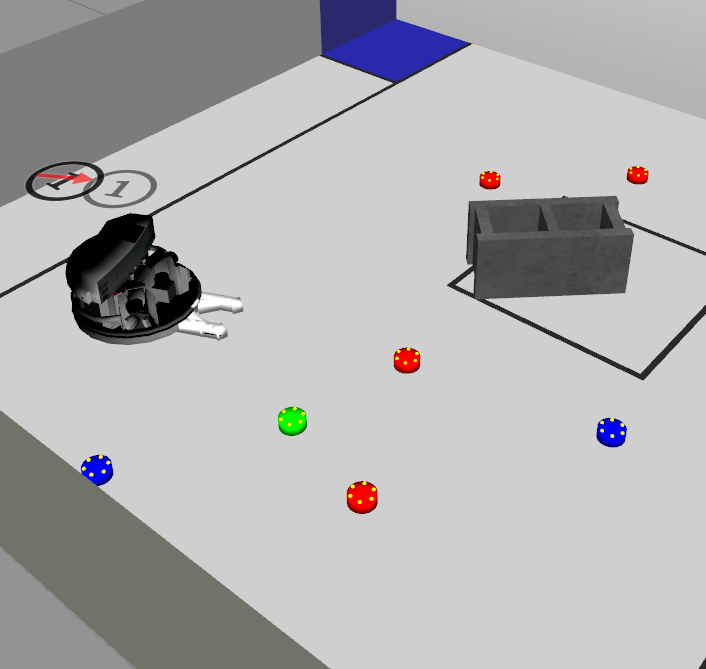
\includegraphics[width=0.3\textwidth]{../pics/hackathon_sim}\\
    \raggedright
    \textbf{\large Bonding Hackathon 2013:}
    \begin{itemize}
    \item $\sim 40$ inexperienced people 
    \item Search and rescue scenario
    \item Possibility of rapid testing with the simulation
    \item Good results
    \item[$\Rightarrow$] Simulation is expandable, easy to use and allows efficient testing
    \end{itemize}
  \end{multicols}
\end{frame}

\begin{frame}
  \frametitle{Evaluation: Agent strategies} % explain configurations
  \begin{multicols}{2}
    \center
    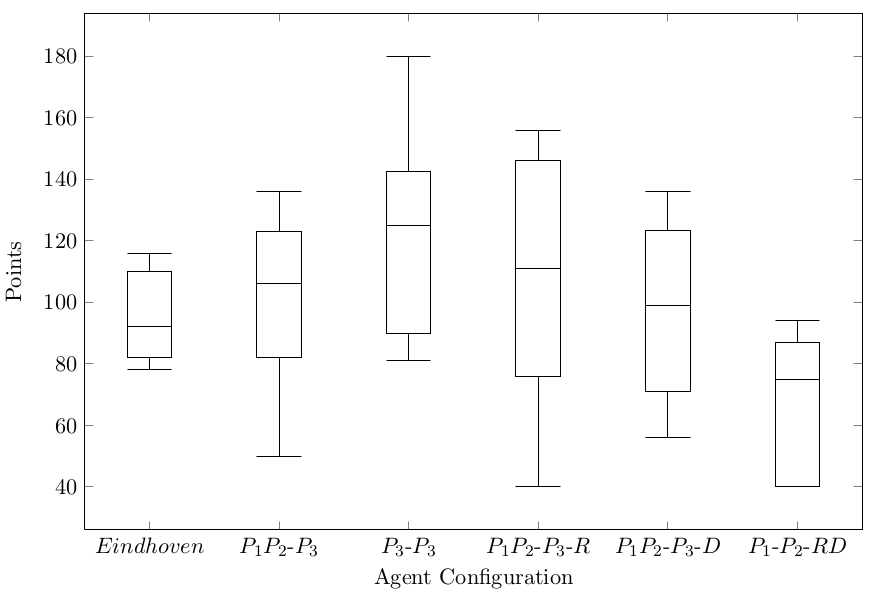
\includegraphics[width=0.47\textwidth]{../pics/eval_two}\\
    %\hspace{0.5cm}\\
    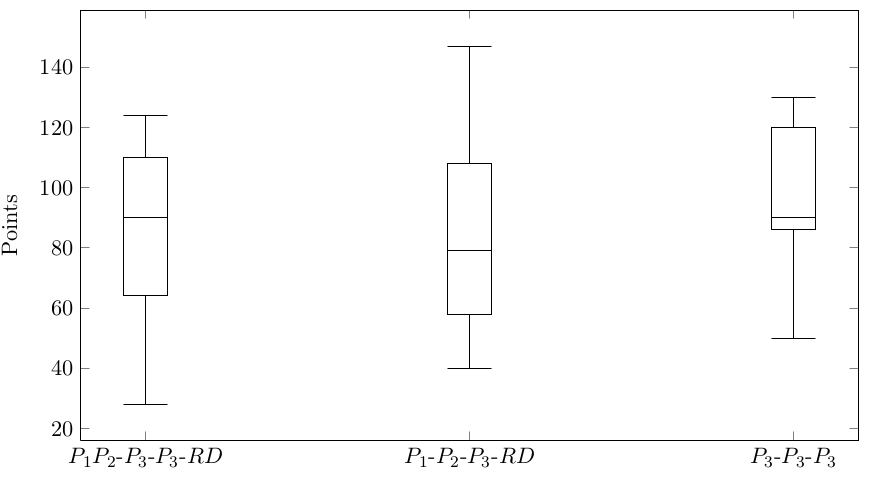
\includegraphics[width=0.47\textwidth]{../pics/eval_three}\\
    \raggedright
    \textbf{\large Evaluation Results:}
    \begin{itemize}
    \item Performance in simulation similar to reality % human interaction + small fixes
    \item $P_3P_3$ performs best % possible in Eindhoven but no possibility to compare strategies
    \item Recycling provides simple points but is more error-prone
    \item Dynamic role change happens only rarely
    \item Uncoordinated navigation and resource bottlenecks limit performance with three agents
    \end{itemize}
  \end{multicols}
\end{frame}

%%%% Summary %%%%

\begin{frame}
  \frametitle{Summary}
  \textbf{\large Multi-robot simulation of LLSF}
  \begin{itemize}
  \item Important to allow efficient testing and developing
  \item Comprehensive simulation of LLSF
  \item Efficient evaluation and comparison of multi-robot strategies
  \item Expandable for future changes
  \item Successfully used in several other developments\\(agent strategies, hackathon, puck-vision, collision-avoidance)
  \end{itemize}
\end{frame}
\end{document}
